\section{Rancangan Solusi}
\label{sec:rancangan-solusi}

\subsection{Gambaran Umum}
Dengan segala kebutuhan yang sudah dianalisis, maka akan dibuat beberapa komponen penyusun sistem yang bisa dilihat pada gambar \ref{fig:rancangan-sistem}. Rencananya, sistem kontrol fleksibel akan dikembangkan dari luar kubernetes cluster sedangkan \textit{Elastic Search} itu sendiri diletakkan didalam kubernetes. Integrasi dengan API \textit{Elastic Search} akan melalui \textit{service} yang disediakan kubernetes sedangkan untuk mengontrol kubernetesnya sendiri akan digunakan \textit{Kubernetes Client Library}.

\begin{figure}[h]
    \centering
    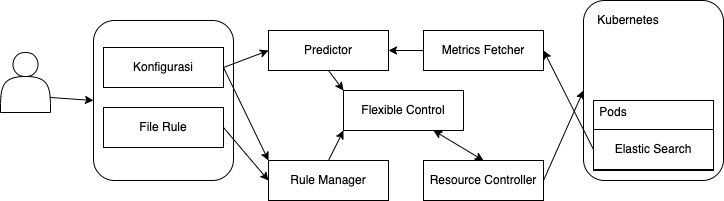
\includegraphics[width=1.1\textwidth]{chapter-3/rancangan.png}
    \caption{Rancangan Komponen Penyusun Sistem}
    \label{fig:rancangan-sistem}
\end{figure}

Sistem kontrol fleksibel dirancangkan akan disusun dari beberapa penyusun, diantaranya sebagai berikut.

\begin{enumerate}
    \item \textbf{Konfigurasi dan \textit{File Rule}}
    
    Konfigurasi dan \textit{File Rule} akan berinteraksi langsung dengan pengguna. Konfigurasi akan dibaca oleh mayoritas komponen sebagai pengaturan terhadap sistem sedangkan file rule yang di\textit{parse} oleh \textit{rule manager} untuk mengatur trigger dari \textit{resource controller} melakukan kontrol fleksibel terhadap alokasi sumber daya.

    \item \textbf{Kubernetes dan \textit{Elastic Search}}
    
    \textit{Elastic Search} akan diletakkan pada sebuah \textit{pods} di dalam sebuah \textit{cluster Kubernetes}. Dibuatkan sebuah \textit{service} agar \textit{Elastic Search} dapat diakses dari luar \textit{cluster}.
    
    \item \textbf{\textit{Predictor}}
    
    \textit{Predictor} akan berisikan model ARIMA untuk setiap variabel yang telah ditentukan. Model-model ini akan digunakan untuk memprediksi nilai variabel pada waktu selanjutnya sesuai permintaan \textit{rule manager}. Karena setiap rule mungkin untuk memiliki keperluan data untuk waktu prediksi yang berbeda.

    \item \textbf{\textit{Metrics Fetcher}}
    
    Komponen \textit{Metrics Fetcher} bertugas untuk menembak \href{https://www.elastic.co/guide/en/elasticsearch/reference/current/cluster-nodes-stats.html}{\textit{Node Stats API}} yang dimiliki oleh \textit{Elastic Search} dan meneruskannya kepada komponen \textit{Predictor} untuk melatih model.

    \item \textbf{\textit{Rule Manager}}
    
    Komponen \textit{Rule Manager} akan melakukan parsing terhadap file rule yang telah diisi oleh pengguna dan mengatur \textit{trigger}. Selain itu, komponen ini akan memberikan informasi tentang waktu prediksi yang diperlukan berdasarkan \textit{rule} yang telah dibuat oleh pengguna.

    \item \textbf{\textit{Resource Controller}}
    
    Komponen \textit{Resource Controller} akan memanfaatkan \textit{Kubernetes Client Library} untuk mengubah spesifikasi \textit{deployment} sehingga alokasi sumber daya dapat berubah. Pada pembuatan komponen ini, harus dilakukan eksperimen \textit{In-place Resource Resize} untuk mengubah alokasi sumber daya tanpa melakukan \textit{restart}.

    \item \textbf{\textit{Flexible Control}}
    
    Komponen \textit{Flexible Control} adalah komponen \textit{high-level} yang akan mengintegrasikan dan mengkolaborasikan komponen-komponen yang disebutkan sebelumnya.
\end{enumerate}

\subsection{Model Prediksi}

Model prediksi yang akan digunakan dalam solusi ini adalah ARIMA. Untuk perbandingan dan penjelasan dengan model-model lain dapat dilihat sebagai berikut.

\begin{enumerate}
    \item \textbf{ARIMA dengan LSTM dan Bi-LSTM}

    ARIMA adalah teknik model prediksi time series yang umum digunakan karena kemudahannya diinterpretasi dan dapat memperhitungkan pola data musiman atau tren yang simpleks. Namun, teknik ARIMA memerlukan banyak pengetahuan tentang data dan dapat memerlukan waktu yang lama untuk membangun model yang baik. Di satu sisi, LSTM yang memakai \textit{neural network} dapat memperhitungkan hubungan yang kompleks antara data historis dan bisa menangani data dengan dimensi yang tinggi. Teknik ini dapat memperhitungkan pola yang berubah dari waktu ke waktu. Kelemahan LSTM sendiri adalah pada kompleksitas perhitungan yang diperlukan untuk membangun model dan interpretasinya yang sulit dari hasil prediksi.

    Secara umum, ARIMA bisa menjadi pilihan yang baik untuk membangun model dengan data yang relatif sederhana dengan kekurangannya adalah waktu yang sangat lama untuk membangun sebuah model. Sedangkan, LSTM merupakah pilihan yang baik apabila data memiliki hubungan yang kompleks dan pola yang berubah dari waktu ke waktu dengan \textit{tradeoff} berupa dibutuhkan percobaan untuk melakukan konfigurasi model serta memikirkan algoritma dan berisiko untuk \textit{overfitting}.

    \item \textbf{ARIMA dengan SARIMA}
    
    Perbedaan dua model ini adalah ARIMA tidak dapat menangkap komponen musiman, sehingga tidak cocok untuk data yang memiliki fluktuasi musiman yang signifikan, seperti data yang bervariasi secara periodik. Di sisi lain, SARIMA adalah pengembangan dari ARIMA yang dapat menangani data dengan komponen musiman. SARIMA memperluas model ARIMA dengan tambahan komponen musiman untuk memodelkan fluktuasi periodik dalam data. Dengan demikian, SARIMA lebih cocok untuk memprediksi pola musiman, seperti data yang meningkat atau menurun secara periodik.

    Dalam hal ini, jika data dapat menunjukkan pola musiman yang jelas seperti faktor cuaca, hari libur, dan sebagainya, lebih tepat untuk menggunakan metode SARIMA. Namun, jika data tersebut cenderung tidak memiliki pola musiman yang kuat, maka metode ARIMA bisa menjadi pilihan yang lebih sederhana dan sesuai.

    \item \textbf{ARIMA dengan VARMAX}
    
    VARMAX adalah pengembangan dari metode VAR (\textit{Vector Autoregression}) yang digunakan untuk data time series multivariat, yang berarti melibatkan lebih dari satu variabel yang saling mempengaruhi. VARMAX memperluas kemampuan VAR dengan menambahkan komponen moving average sehingga dapat memodelkan hubungan yang lebih kompleks antara berbagai variabel. Sehingga, apabila data melibatkan banyak variabel yang saling mempengaruhi, maka VARMAX sangat cocok untuk dipakai karena VARMAX mempertimbangkan kompleksitas dan hubungan antar variabel.

\end{enumerate}

Oleh karena ini, pada tugas akhir ini pemakaian ARIMA didasari atas konsiderasi pada poin berikut.

\begin{enumerate}
    \item ARIMA lebih sederhana dibandingkan dengan LSTM dan Bi-LSTM.
    \item SARIMA membutuhkan pola musiman data yang jelas, yang tidak bisa dipastikan saat penulisan tugas akhir.
    \item Tidak ada keperluan untuk melibatkan hubungan antar variabel.
\end{enumerate}

\subsection{Sistem \textit{Rule}}

Dalam melakukan pemasangan \textit{autoscaler}, umumnya pengelola akan melakukan pengubahan \textit{treshold} dan jumlah \textit{request} serta \textit{limit} sumber daya untuk sebuah \textit{pods}. Apabila suatu saat terdapat perubahan pola penggunaan, maka pengelola harus menyesuaikan konfigurasi tersebut. Hal ini dapat dilakukan dengan cara memonitoring \textit{cluster} secara berkala dan melakukan perubahan konfigurasi secara manual. Namun, hal ini akan memakan waktu dan tenaga yang tidak sedikit. Oleh karena itu, dibutuhkan sebuah sistem yang dapat melakukan perubahan konfigurasi secara otomatis berdasarkan pola penggunaan yang terjadi. Secara umum, sistem \textit{rule} yang akan dibuat akan memiliki fungsional sebagai berikut.

\begin{enumerate}
    \item Terdapat beberapa kondisi yang dapat melakukan \textit{trigger} scaling.
    \item Terdapat sebuah konfigurasi aksi yang akan dilakukan apabila kondisi terpenuhi.
    \item Terdapat variabel \textit{user-defined} yang bisa digunakan oleh pengguna untuk perantara antar kondisi atau menggabungkan beberapa kondisi atau menjadi \textit{dynamic treshold} karena kondisi lain terpenuhi.
\end{enumerate}

\subsection{Arsitektur Sistem}

Arsitektur sistem akan mengikuti \textbf{MAPE Loop} yang direferensikan dari riset terkait, \parencite{riset1}. Gambar arsitektur ini bisa dilihat pada gambar \ref{fig:mape}. Berikut adalah rancangan fase dengan arsitektur tersebut.

\begin{enumerate}
    \item \bfseries \textit{Monitor} \normalfont
    
        Fase ini akan menarik data dari \textit{Application Metric Collector}, yang pada konteks tugas akhir ini akan menarik dari \textit{Node Stats API} milik \textit{Elastic Search}.
    \item \bfseries \textit{Analyse} \normalfont
    
        Model prediksi akan memanfaatkan data yang didapat dari fase sebelumnya untuk melakukan analisa dan prediksi yang akan datang. Setelah berhasil memproses data tersebut, fase dilanjutkan ke fase \textit{Planning}.
    \item \bfseries \textit{Planning} \normalfont
    
        Fase ini akan melakukan pengecekan semua kondisi yang telah dikonfigurasi oleh pengelola. Pertama-tama, sistem akan melihat semua kebutuhan variabel prediksi. Lalu melakukan prediksi dengan menggunakan model prediksi yang sudah dibangun. Setelah itu, sistem akan melakukan pengecekan kondisi satu per satu. Apabila kondisi terpenuhi, maka sistem akan melakukan aksi yang telah dikonfigurasi ke dalam antrian yang akan dieksekusi pada fase berikutnya. Setelah semua kondisi dicek, maka fase dilanjutkan ke fase \textit{Execution}.
    \item \bfseries \textit{Execution} \normalfont
    
        Fase ini akan melakukan eksekusi perubahan alokasi sumber daya apabila diperlukan. Apabila tidak memerlukan pengubahan alokasi sumber daya, maka akan dilanjutkan dengan mengulang ke fase \textit{Monitor} pada \textit{loop} berikutnya.
\end{enumerate}

\subsection{Rancangan Kelas Penyusun Sistem dan Spesifikasi Kelas}

\subsection{Alur Kerja Sistem}

Untuk alur kerja sistem, secara spesifik \textit{autoscaler} dengan kontrol fleksibel akan melakukan tugasnya dengan alur yang bisa dilihat pada gambar XXX.